\documentclass[12pt,reqno]{amsart}\usepackage[]{graphicx}\usepackage[]{color}
%% maxwidth is the original width if it is less than linewidth
%% otherwise use linewidth (to make sure the graphics do not exceed the margin)
\makeatletter
\def\maxwidth{ %
  \ifdim\Gin@nat@width>\linewidth
    \linewidth
  \else
    \Gin@nat@width
  \fi
}
\makeatother

\definecolor{fgcolor}{rgb}{0.345, 0.345, 0.345}
\newcommand{\hlnum}[1]{\textcolor[rgb]{0.686,0.059,0.569}{#1}}%
\newcommand{\hlstr}[1]{\textcolor[rgb]{0.192,0.494,0.8}{#1}}%
\newcommand{\hlcom}[1]{\textcolor[rgb]{0.678,0.584,0.686}{\textit{#1}}}%
\newcommand{\hlopt}[1]{\textcolor[rgb]{0,0,0}{#1}}%
\newcommand{\hlstd}[1]{\textcolor[rgb]{0.345,0.345,0.345}{#1}}%
\newcommand{\hlkwa}[1]{\textcolor[rgb]{0.161,0.373,0.58}{\textbf{#1}}}%
\newcommand{\hlkwb}[1]{\textcolor[rgb]{0.69,0.353,0.396}{#1}}%
\newcommand{\hlkwc}[1]{\textcolor[rgb]{0.333,0.667,0.333}{#1}}%
\newcommand{\hlkwd}[1]{\textcolor[rgb]{0.737,0.353,0.396}{\textbf{#1}}}%

\usepackage{framed}
\makeatletter
\newenvironment{kframe}{%
 \def\at@end@of@kframe{}%
 \ifinner\ifhmode%
  \def\at@end@of@kframe{\end{minipage}}%
  \begin{minipage}{\columnwidth}%
 \fi\fi%
 \def\FrameCommand##1{\hskip\@totalleftmargin \hskip-\fboxsep
 \colorbox{shadecolor}{##1}\hskip-\fboxsep
     % There is no \\@totalrightmargin, so:
     \hskip-\linewidth \hskip-\@totalleftmargin \hskip\columnwidth}%
 \MakeFramed {\advance\hsize-\width
   \@totalleftmargin\z@ \linewidth\hsize
   \@setminipage}}%
 {\par\unskip\endMakeFramed%
 \at@end@of@kframe}
\makeatother

\definecolor{shadecolor}{rgb}{.97, .97, .97}
\definecolor{messagecolor}{rgb}{0, 0, 0}
\definecolor{warningcolor}{rgb}{1, 0, 1}
\definecolor{errorcolor}{rgb}{1, 0, 0}
\newenvironment{knitrout}{}{} % an empty environment to be redefined in TeX

\usepackage{alltt}
\usepackage{geometry}                % See geometry.pdf to learn the layout options. There are lots.
\geometry{letterpaper}                   % ... or a4paper or a5paper or ... 
%\geometry{landscape}                % Activate for for rotated page geometry
%\usepackage[parfill]{parskip}    % Activate to begin paragraphs with an empty line rather than an indent
\usepackage{graphicx}
\usepackage{amsfonts}
\usepackage{amsthm}
\usepackage{epstopdf}
\usepackage{hyperref}
\usepackage{enumerate}

%Fix \mathbb
\DeclareFontFamily{U}{futm}{}
\DeclareFontShape{U}{futm}{m}{n}{
  <-> s * [.92] fourier-bb
  }{}
\DeclareSymbolFont{Ufutm}{U}{futm}{m}{n}
\DeclareSymbolFontAlphabet{\mathbb}{Ufutm}

%language packages
\usepackage[utf8]{inputenc}
\usepackage[spanish]{babel}

%color packages
\usepackage{amsmath,color,graphicx}
\definecolor{myred}{rgb}{0.6,0,0} 



%Include definitions
%% Place here your \newcommand's and \renewcommand's. Some examples already included.
%%
\renewcommand{\le}{\leqslant}
\renewcommand{\ge}{\geqslant}
\renewcommand{\emptyset}{\ensuremath{\varnothing}}
\newcommand{\ds}{\displaystyle}
\newcommand{\R}{\ensuremath{\mathbb{R}}}
\newcommand{\Q}{\ensuremath{\mathbb{Q}}}
\newcommand{\Z}{\ensuremath{\mathbb{Z}}}
\newcommand{\N}{\ensuremath{\mathbb{N}}}
\newcommand{\T}{\ensuremath{\mathbb{T}}}
\newcommand{\eps}{\varepsilon}
\newcommand{\closure}[1]{\ensuremath{\overline{#1}}}

%MINE
%\newcommand{\norm}[1]{\left\Vert#1\right\Vert}
%\newcommand{\abs}[1]{\left\vert#1\right\vert}
\newcommand{\set}[1]{\left\{#1\right\}}
\newcommand{\epsi}{\varepsilon}
\newcommand{\To}{\longrightarrow}
\newcommand{\BX}{\mathbf{B}(X)}
\newcommand{\A}{\mathcal{A}}
\newcommand{\St}{\mathcal{S}}
\newcommand{\Par}{\mathcal{P}}
\newcommand{\La}{\mathcal{L}}
\newcommand{\F}{\mathcal{F}}

%LINEAR ALGEBRA
\newcommand{\tr}{\mathrm{tr}}
\newcommand{\sign}{\mathrm{sign}}
\providecommand{\norm}[1]{\lVert#1\rVert}

%PROBABILITY
\newcommand{\Var}{\mathrm{Var}\:}
\newcommand{\Cov}{\mathrm{Cov}\:}
\newcommand{\dis}{\mathrm{d}}

%Numerics
\newcommand{\Fb}{\textbf{F}}

%Theorem Styles
\newtheorem{thm}{Theorem}[section]
\newtheorem{cor}[thm]{Corollary}
\newtheorem{lem}[thm]{Lemma}

\theoremstyle{remark}
\newtheorem{rem}[thm]{Remark}

%Mattias
\newcommand{\mpar}[1]{{\marginpar{\tiny #1}}}
\newcommand{\notto}{\nrightarrow}
\newcommand{\Lloc}{L^1_{\mathrm{loc}}}
\newcommand{\Ito}{It{\^o}\ }
\newcommand{\Itos}{It{\^o}'s\ }
\newcommand{\eg}{e.g.\ }
\newcommand{\ie}{i.e.\ }
\newcommand{\as}{a.s.\ }
\newcommand{\iid}{i.i.d.\ }
\newcommand{\qand}{{\quad\text{and}\quad}}
\newcommand{\qor}{{\quad\text{or}\quad}}
\newcommand{\fixme}{{\begin{center}{\textbf{\huge fixme}}\end{center}}}
\newcommand{\work}{{\begin{center}{\textbf{\huge work}}\end{center}}}
\newcommand{\smilie}{{$:\hspace{-1mm}-\hspace{-0.5mm})$}}
\newcommand{\pa}{{\partial}}

%\newcommand{\acim}{\textsc{acim}\xspace}
%\newcommand{\acims}{\textsc{acim}s\xspace}

%%
%% Place here your \newtheorem's:
%%

%% Some examples commented out below. Create your own or use these...
%%%%%%%%%\swapnumbers % this makes the numbers appear before the statement name.
%\theoremstyle{plain}
%\newtheorem{thm}{Theorem}[chapter]
%\newtheorem{prop}[thm]{Proposition}
%\newtheorem{lemma}[thm]{Lemma}
%\newtheorem{cor}[thm]{Corollary}

%\theoremstyle{definition}
%\newtheorem{define}{Definition}[chapter]

%\theoremstyle{remark}
%\newtheorem*{rmk*}{Remark}
%\newtheorem*{rmks*}{Remarks}

%% This defines the "proo" environment, which is the same as proof, but
%% with "Proof:" instead of "Proof.". I prefer the former.
%\newenvironment{proo}{\begin{proof}[Proof:]}{\end{proof}}


\DeclareGraphicsRule{.tif}{png}{.png}{`convert #1 `dirname #1`/`basename #1 .tif`.png}

\title{Principales variables aleatorias.}
\author{Vidal Alcalá}
%\date{}                                           % Activate to display a given date or no date
\IfFileExists{upquote.sty}{\usepackage{upquote}}{}
\begin{document}

\maketitle

A continuación describiremos las distribuciones básicas junto con su simulación en el lenguaje \verb+R + .

% \section{Distribución uniforme}
% La variable aleatoria $X$ tiene densidad uniforme en el intervalo $[a,b]$ si
% \begin{equation*}
%   \begin{split}
%   P(X\in [r,s]) &= \frac{r - s}{b-a},\qquad a< r \leq s < b \:.
% 	\end{split}
% \end{equation*}
% Se sigue que la probabilidad de que $X$ pertenezca a un intervalo no depende de la posición del intervalo y solo depende de la longitud del intervalo. En términos de funciones de distribución y densidad tenemos
% \begin{equation}\label{disUniforme}
%   \begin{split}
%   F(x) &= P(X \leq x) = \begin{cases}
%            0 & x < a\\
%            \frac{x-a}{b-a} & a\leq x \leq b\\
%            1 & b < x
% 	        \end{cases}
%   \end{split}
% \end{equation}
% \begin{equation}\label{denUniforme}
%   \begin{split}
%   f(x) &=F'(x)= \begin{cases}
%            0 & x < a\\
%            \frac{1}{b-a} & a\leq x \leq b\\
%            1 & b < x\:.
%           \end{cases}
%   \end{split}
% \end{equation}
% Escribiremos $X \sim U(a,b)$ para denotar que la variable aleatoria $X$ tiene distribución uniforme en el intervalo $(0,1)$. El siguiente código genera 10000 muestras $U(1,3)$ y se dibuja el histograma.
% << GeneraU >>=
% ##parametros
% L = 10000
% a <- 1
% b <- 3
% x <- runif(L,a,b)
% @
% << hist , fig.width=4,fig.height=4,out.width='.60\\linewidth' , tidy=FALSE >>=
% xHist <- hist(x, prob = TRUE , breaks = 10*log(L))
% f <- function(x) rep( 1.0 / (b-a) , length(x) )
% curve( f , xHist$mids[1] , xHist$mids[length(xHist$mids)] ,
%        add = TRUE, col = 'red')
% @
% 
% \section{Distribución triangular}
% La variable aleatoria $X$ tiene distribución triangular si su función de densidad es la siguiente.
% \begin{equation}\label{denTriangular}
%   \begin{split}
%   f(x) &=\begin{cases}
%     0 & \text{si } 0\leq x\leq a\\
% 	  4\frac{x-a}{(b-a)^2} & \text{si } a < x \leq \frac{a+b}{2}\\
% 	  -4\frac{x-b}{(b-a)^2} & \text{si } \frac{a+b}{2} < x \leq b \\
% 	  0 & \text{si } b< x
% 	  \end{cases}
%   \end{split}
% \end{equation}
% Escribiremos $X \sim T(a,b)$ para denotar que la variable aleatoria $X$ tiene distribución triangular en el intervalo $(a,b)$. El siguiente código genera 10000 muestras $T(1,3)$ y dibuja el histograma.
% << GeneraT ,  tidy=FALSE>>=
% ##parametros
% L = 10000
% a <- 1
% b <- 3
% u <- runif(L)
% Finv <- function( u ) ifelse( u < 0.5 ,
%                               a + (b-a)*sqrt(u/2.0) ,
%                               b - (b-a)*sqrt( ( 1.0 - u )/2.0) ) 
% x = Finv(u)
% @
% << histT , fig.width=4,fig.height=4,out.width='.60\\linewidth' , tidy=FALSE >>=
% xHist <- hist(x, prob = TRUE, breaks = 10*log(L) )
% f <- function(x) ifelse ( (x < b) & (a < x) ,
%                           ifelse ( x < ( a + b )/2.0 ,
%                                    4* (x-a)/(b-a)^2 ,
%                                    -4* (x-b)/(b-a)^2 ) ,
%                           rep( 0 , length(x) )
%                           )
% curve( f , xHist$mids[1] , xHist$mids[length(xHist$mids)] ,
%        add = TRUE, col = 'red')
% @
% \section{Funciones de densidad conjunta}
% La función de densidad conjunta de dos variables aleatorias $X$ y $Y$ la vamos a denotar por $f(x,y)$. La propiedad que la define es que para cualquier conjunto $A\subset \R^2$ tenemos
% \begin{equation}\label{denConjunta}
%   \begin{split}
%   P((X,Y)\in A) &= \int_{A} f(x,y)|dxdy|\:.
%   \end{split}
% \end{equation}
% Por ejemplo, si $A = \set{(x,y)|x<y}$ entonces
% \begin{equation}
%   \begin{split}
%   P(X<Y) &= \int_{x<y} f(x,y)|dxdy| \\
%   &= \int_{-\infty}^{\infty}\biggl( \int_{-\infty}^{y}f(x,y) dx \biggr) dy  \:.
%   \end{split}
% \end{equation}
% 
% \begin{thm}
% Las variables aleatorias $X$ y $Y$ son independientes sii la función de densidad conjunta se puede escribir como el producto de una función de solo $x$ y una función de solo $y$, es decir
% \begin{equation}\label{denIndependiente}
%   \begin{split}
%  f(x,y) &= g(x)h(y)\:.
%   \end{split}
% \end{equation}
% Más aún, en este caso $g(x)\propto f_{X}(x)$ y $h(y)\propto f_{Y}(y)$. 
% \end{thm}
% 
% Podemos calcular la función de densidad marginal de X en términos de la función de densidad conjunta de la siguiente manera. Primero calculamos la función de distribución.
% \begin{equation*}
%   \begin{split}
%   F_{X}(x) &=  P(X < x) \\
%   &= \int_{z<x} f(z,w)|dzdw| \\
%   &= \int_{-\infty}^{x}\biggl( \int_{-\infty}^{\infty}f(z,w) dw \biggr) dz  \\
%   \end{split}
% \end{equation*}
% Ahora usamos el Teorema Fundamental del Cálculo para calcular la derivada.
% \begin{equation}
%   \begin{split}
%   f_{X}(x) &=  \frac{d}{dx}F(x) \\
%   &=\frac{d}{dx} \int_{-\infty}^{x}\biggl( \int_{-\infty}^{\infty}f(z,w) dw \biggr) dz  \\
%   &=\int_{-\infty}^{\infty}f(x,w) dw \:.
%   \end{split}
% \end{equation}
% 
% \section{Álgebra lineal}
% Algunas propiedades de las matrices que vamos a utilizar. Sean $A$ y $B$ matrices de $n\times n$ y $v$ un vector columna en $\R^n$.
% \begin{equation}\label{algLineal}
%   \begin{split}
%    (AB)^{T} &= B^T A^T \\
%    (AB)^{-1} &= B^{-1} A^{-1} \\
%    \det(AB) &= \det A \det B \\
%    \det(A^T) &= \det (A)\\
%    v^T v &= v_1^2+v_2^2+\ldots+v_n^2\:.
%   \end{split}
% \end{equation}
% 
% 
% 
% 
% \section{Distribución normal}
% La distribución normal es la más importante en el el estudio de procesos financieros. Su ubicuidad se debe al teorema del límite central y a la independencia de los rendimientos de un activo sobre intervalos de tiempo disjuntos. Discutiremos esta relación más adelante en el curso y por lo pronto estudiaremos sus propiedades.
% 
% La variable aleatoria $X$ tiene distribución normal con media $\mu$ y varianza $\sigma^2$ si su función de densidad es 
% \begin{equation}\label{denNormal}
%   \begin{split}
%   f(x) &= \frac{\exp(-\frac{(x-\mu)^2}{2 \sigma^2})}{\sqrt{2 \pi \sigma^2}}\:.
%   \end{split}
% \end{equation}
% Escribiremos $X \sim N(\mu,\sigma^2)$ para denotar que la variable aleatoria $X$ tiene la densidad anterior. El siguiente código genera 10,000 muestras $N(3,4)$ y dibuja el histograma. Nótese que en el lenguaje \verb+ R + el parámetro que se usa es la desviación estándar $\sigma$.
% << GeneraN >>=
% ##parametros
% L = 10000
% mu <- 3.0
% sigma <- 2.0
% x <- rnorm(L,mu,sigma)
% @
% << histN , fig.width=4,fig.height=4,out.width='.60\\linewidth' , tidy=FALSE >>=
% xHist <- hist(x, prob = TRUE , breaks = 10*log(L))
% f <- function(x) exp(- ((x-mu)^2)/(2*sigma^2))/sqrt(2*pi*sigma^2)
% curve( f , xHist$mids[1] , xHist$mids[length(xHist$mids)] ,
%        add = TRUE, col = 'red')
% @
% 
% La distribución normal tiene una extensión natural para el caso de variables aleatorias correlacionadas. Supongamos que $Z_1,Z_2$ son variables aleatorias normales estándar independientes. Acomodamos las v.a. en un vector columna $Z = (Z_1,Z_2)^T$ y definimos un vector aleatorio $X$ mediante una transformación lineal $\sigma: \R^2 \to \R^2$, es decir $X = \sigma Z$. En términos de las coordenadas del vector $X$ tenemos
% \begin{equation}\label{coordenadasX}
%   \begin{split}
%   X_1 &= \sigma_{11}Z_1 + \sigma_{12}Z_2\\
%   X_2 &= \sigma_{21}Z_1 + \sigma_{22}Z_2\\
%   \end{split}
% \end{equation}
% Las entradas de $X$ no son independientes porque en las sumas que las definen hay elementos repetidos. Podemos calcular la covarianza entre las entradas como sigue.
% \begin{equation*}
%   \begin{split}
%   \Cov(X_1 ,X_2) &=\Cov(\sigma_{11}Z_1 + \sigma_{12}Z_2,\sigma_{21}Z_1 + \sigma_{22}Z_2 )\\
%  &= \sum_{k,l}\sigma_{1k}\sigma_{2l}\Cov(Z_k,Z_l)
%   \end{split}
% \end{equation*}
% Usando que las v.a. $Z_i$ son independientes y tienen varianza 1 obtenemos que
% \begin{equation}\label{covarianzaX12}
%   \begin{split}
%   \Cov(X_1 ,X_2) &=\sum_{k}\sigma_{1k}\sigma_{2k}
%   \end{split}
% \end{equation}
% La suma que aparece al final de la última ecuación es igual a la entrada $(1,2)$ de la matriz $\sigma\sigma^T$. Cálculos similares llevan a la conclusión de que la \emph{matriz de covarianza} de $X$ es $\Sigma = \sigma\sigma^T$. En otras palabras
% \begin{equation}\label{covarianzaX}
%   \begin{split}
%   \Cov(X_i ,X_j) &=\sum_{k}\sigma_{ik}\sigma_{jk}=(\sigma\sigma^T)_{ij}\:.
%   \end{split}
% \end{equation}
% 
% 
% También podemos calcular la función de densidad del vector $X$ de la siguiente forma.
% \begin{enumerate}
% \item Escribir la función de densidad de $Z$ en \emph{notación diferencial}.
% \begin{equation}\label{density_z}
%   \begin{split}
%   f_{Z}(z) |dz| &= \frac{e^{-z_1^2/2}}{\sqrt{2\pi}}\frac{e^{-z_2^2/2}}{\sqrt{2\pi}} |dz_1 dz_2|\\
%   &= \frac{e^{-\frac{1}{2}z^T z}}{\sqrt{2\pi}} |dz_1 dz_2|\:.
%   \end{split}
% \end{equation}
% \item Sustituir $z_i$ y $dz_i$ en la ecuación anterior usando la relación $x = \sigma z$. 
% Despejando $z$ obtenemos
% \begin{equation}\label{z}
%   \begin{split}
%   z &= \sigma^{-1} x,  
%   \end{split}
% \end{equation}
% Calculando el diferencial obtenemos
% \begin{equation*}
%   \begin{split}
%   dx_1 &= \sigma_{11}dz_1 + \sigma_{12}dz_2\\
%   dx_2 &= \sigma_{21}dz_1 + \sigma_{22}dz_2\:.
%   \end{split}
% \end{equation*}
% Usando que $dz_1 dz_1=0$, $dz_2 dz_2=0$ y  $dz_1 dz_2 = - dz_2 dz_1$ calculamos
% \begin{equation}\label{dz}
%   \begin{split}
%   dx_1 dx_2 &= \sigma_{11}\sigma_{22}dz_1 dz_2 + \sigma_{12}\sigma_{21} dz_2 dz_1\\
%   &= (\sigma_{11}\sigma_{22}-  \sigma_{12}\sigma_{21})dz_1dz_2\\
%   &= \det(\sigma) dz_1 dz_2\\
%   \end{split}
% \end{equation}
% Finalmente sustituimos \eqref{z} y \eqref{dz} en la ecuación \eqref{density_z} para obtener
% \begin{equation}\label{substitute_x}
%   \begin{split}
%   f_{Z}(z) |dz| &= \frac{e^{-\frac{1}{2}x^T(\sigma\sigma^T)^{-1}x}}{(\sqrt{2\pi})^2}\frac{1}{|\det{\sigma}|} |dx_1 dx_2|\:.
%   \end{split}
% \end{equation}
% \item El factor enfrente de $|dx_1 dx_2|$ es la función de densidad de la variable aleatoria $X$, en otras palabras
% \begin{equation}\label{density_x}
%   \begin{split}
%   f_{X}(x) &= \frac{e^{-\frac{1}{2}x^T(\sigma\sigma^T)^{-1}x}}{(\sqrt{2\pi})^2}\frac{1}{|\det{\sigma}|}\:.
%   \end{split}
% \end{equation}
% \end{enumerate}
% Usando propiedades básicas del determinante de una matriz podemos calcular
% \begin{equation*}
%   \begin{split}
%   \det(\sigma \sigma^T) &= \det(\sigma) \det(\sigma^T)\\
%   &= \det(\sigma) \det(\sigma)\\
%   &= \det(\sigma)^2\:.
%   \end{split}
% \end{equation*}
% En términos de la matriz $\Sigma$ hemos obtenido que
% \begin{equation*}
%   \begin{split}
%   f_{X}(x) &= \frac{e^{-\frac{1}{2}x^T \Sigma ^{-1}x}}{(\sqrt{2\pi})^2}\frac{1}{\sqrt{\det{\Sigma}}}\:.
%   \end{split}
% \end{equation*}
% En el caso multivariado donde $X\in \R^n$ y $\sigma:\R^n\To \R^n$ la ecuación anterior se convierte en
% \begin{equation}\label{density_N}
%   \begin{split}
%   f_{X}(x) &= \frac{e^{-\frac{1}{2}x^T \Sigma ^{-1}x}}{(\sqrt{2\pi})^n\sqrt{\det{\Sigma}}}\:.
%   \end{split}
% \end{equation}
% En este caso decimos que las entradas $X_i$ tienen una \emph{distribución normal conjunta} con media cero y covarianza $\Sigma$. Si queremos que $E[X_i]=\mu_i$ la función de densidad debe ser
% \begin{equation}\label{density_N_mu}
%   \begin{split}
%   f_{X}(x) &= \frac{e^{-\frac{1}{2}(x-\mu)^T \Sigma ^{-1}(x-\mu)}}{(\sqrt{2\pi})^n\sqrt{\det{\Sigma}}}\:.
%   \end{split}
% \end{equation}
% 
% \section{Método Box-Muller}
% Una aplicación interesante de variables normales conjuntas se obtiene mediante el cambio de coordenadas polar
% \begin{equation}\label{polar}
%   \begin{split}
%   Z_1 &= R \cos \Theta\\
%   Z_2 &= R \sin \Theta\:,
%   \end{split}
% \end{equation}
% con $0\leq R$ y $0\leq \Theta < 2\pi$. Calculamos la función de densidad conjunta de $R$ y $\Theta$ a continuación.
% \begin{enumerate}
% \item Escribir la función de densidad de $Z$ en \emph{notación diferencial}.
% \begin{equation}
%   \begin{split}
%   f_{Z}(z) |dz| &= \frac{e^{-z_1^2/2}}{\sqrt{2\pi}}\frac{e^{-z_2^2/2}}{\sqrt{2\pi}} |dz_1 dz_2|\\
%   &= \frac{e^{-\frac{1}{2}z^T z}}{(\sqrt{2\pi})^2} |dz_1 dz_2|\:.
%   \end{split}
% \end{equation}
% \item Sustituir $z_i$ y $dz_i$ en la ecuación anterior usando las ecuaciones \eqref{polar}.
% Calculando el diferencial obtenemos
% \begin{equation*}
%   \begin{split}
%   dz_1 &= - r \sin \theta d\theta + \cos \theta dr\\
%   dz_2 &= r \cos \theta d\theta + \sin \theta dr\\
%   \end{split}
% \end{equation*}
% Usando que $dr dr=0$, $d\theta d\theta=0$ y  $dr d\theta = - d\theta dr$ calculamos
% \begin{equation}\label{dr}
%   \begin{split}
%   dz_1 dz_2 &= - r \sin^2 \theta  d\theta dr + r  \cos^2 \theta  dr d\theta \\
%   &= - r \sin^2 \theta  d\theta dr - r  \cos^2 \theta d\theta dr \\
%   &= r dr d\theta\\
%   \end{split}
% \end{equation}
% Finalmente sustituimos \eqref{polar} y \eqref{dr} en la ecuación \eqref{density_z} para obtener
% \begin{equation}\label{substitute_r}
%   \begin{split}
%   f_{Z}(z) |dz| &= r |dr d\theta| \:.
%   \end{split}
% \end{equation}
% \item El factor enfrente de $|dr d\theta |$ es la función de densidad conjunta de las variables aleatorias $R$ y $\Theta$, en otras palabras
% \begin{equation}\label{density_r}
%   \begin{split}
%   f_{R,\Theta}(r,\theta) &= \frac{r\:e^{-\frac{1}{2}r^2}}{2\pi}\:.
%   \end{split}
% \end{equation}
% \end{enumerate}
% La función de densidad conjunta \eqref{density_r} es el producto de las funciones de densidad $f_{R}(r) = r\:e^{-\frac{1}{2}r^2}$ y $f_{\Theta}(\theta) = \frac{1}{2\pi}$ y por lo tanto $R$ y $\Theta$ son independientes. Suponiendo que $U_1$ y $U_2$ son v.a. $U(0,1)$ e independientes obtenemos que $ R = \sqrt{-2\log U_1} $ y $\Theta = 2\pi U_2$ son v.a. independientes con funciones de densidad $f_R$ y $f_{\Theta}$, respectivamente. Finalmente, $Z_1 = R\cos \Theta$ y $Z_2 = R \sin \Theta$ son v.a. normales estándar e independientes.
% 
% \section{Distribución exponencial}
% La distribución exponencial con parámetro $\lambda$ tiene función de densidad
% \begin{equation}\label{dexp}
%   \begin{split}
%   f(t)&= \lambda \exp(-\lambda t),\qquad t > 0 \:,
%   \end{split}
% \end{equation}
% 
% y función de distribución
% \begin{equation}\label{pexp}
%   \begin{split}
%   F(t)&= 1-\exp(-\lambda t),\qquad t > 0 \:.
%   \end{split}
% \end{equation}
% Su valor esperado y varianza están dados por
% \begin{equation}\label{mexp}
%   \begin{split}
%   E[T] &= \frac{1}{\lambda}\\
%   \Var [T] &=\frac{1}{\lambda^2} \\
%   \end{split}
% \end{equation}
% Esta distribución se utiliza para modelar tiempos de espera. Una propiedad deseable para la distribución de un tiempo de espera es que el tiempo de espera sea el mismo sin importar el tiempo que se ha esperado. En notación de probabilidades condicionales esto se escribe
% \begin{equation}\label{prop_exp}
%   \begin{split}
%     P(T \leq t | T > s ) &= P( T \leq t-s)\\
%     \frac{P(T \leq t , T > s )}{P(T>s)} &= P( T \leq t-s)\\
%     \frac{\int_{s}^{t} f(x) dx}{\int_{s}^{\infty}f(x)dx} &= \int_{0}^{t-s}f(x)dx\:.
%   \end{split}
% \end{equation}
% Tomamos la derivada con respecto de $t$ en la ecuación anterior para obtener
% \begin{equation}
%   \begin{split}
%     \frac{f(t)}{\int_{s}^{\infty}f(x)dx} &= f(t-s)\\
%     f(t)&= f(t-s)\int_{s}^{\infty}f(x)dx\\
%   \end{split}
% \end{equation}
% Finalmente tomamos la derivada con respecto de $s$ en la ecuación anterior para obtener
% \begin{equation}
%   \begin{split}
%     0 &= -f'(t-s)\int_{s}^{\infty}f(x)dx -f(t-s)f(s) \:,
%   \end{split}
% \end{equation}
% y evaluando en $s=0$ la ecuación anterior se convierte en
% \begin{equation}
%   \begin{split}
%     f'(t) &=-f(0)f(t) ,\qquad t>0\:.
%   \end{split}
% \end{equation}
% La solución de la ecuación diferencial anterior es $f(t)=C\exp(-f(0)t)$ y si denotamos $\lambda=f(0)$ obtenemos que $C=\lambda$.
% 
% \section{Distribución de Erlang}
% La suma de variables aleatorias exponenciales independientes $T_1,T_2$ \emph{no es exponencial}. De hecho, podemos calcular
% \begin{equation}
%   \begin{split}
%     P(T_1+T_2 < t) &= \int_{0}^{t} \int_{0}^{t-t_1} \lambda^2 \exp(-\lambda (t_1+t_2)) d t_2 t_1\\
%     &= \int_{0}^{t} \int_{0}^{t-t_1} \lambda^2 \exp(-\lambda (t_1+t_2)) d t_2 d t_1\\
%     &= -\lambda \exp(-\lambda t) t - \exp(-\lambda t) + 1\\
%     \frac{d}{dt}P(T_1+T_2 < t) &= \lambda^2 \exp(-\lambda t ) t\:.
%   \end{split}
% \end{equation}
% Se sigue que la función de densidad de $T_1+T_2$ es $f_{T_1+T_2}(t)=  \lambda^2 \exp(-\lambda t ) t$. En general se puede probar que
% \begin{equation}\label{derlang}
%   \begin{split}
%     f_{T_1+T_2 +\ldots + T_k}(t) &=\frac{\lambda^{k} \exp(-\lambda t ) t^{k-1} }{(k-1)!}\:.
%   \end{split}
% \end{equation}
% Esta es la densidad de Erlang con parámetros $k$ y $\lambda$. El valor esperado y la varianza se calculan a continuación.
% \begin{equation}\label{merlang}
%   \begin{split}
%     E[T_1+T_2 +\ldots + T_k] &= \frac{k}{\lambda}\\
%     \Var [T_1+T_2 +\ldots + T_k] &= \frac{k}{\lambda^2}\:.
%   \end{split}
% \end{equation}
% La simulación en \verb+ R + de la distribución de Erlang se hace mediante la distribución Gamma con densidad
% \begin{equation}\label{dgamma}
%   \begin{split}
%     f(x) &=\frac{s^{-a} \exp(-\frac{x}{s} ) x^{a-1} }{\Gamma(a)}\:.
%   \end{split}
% \end{equation}
% Las muestras se crean llamando \verb+ rgamma ( L , shape = a , scale = s ) +.
% << GeneraErlang >>=
% ##parametros
% L = 10000
% lambda <- 0.25
% k <- 3
% x <- rgamma( L , shape = k , scale = 1.0/lambda )
% @
% << histErlang , fig.width=4,fig.height=4,out.width='.60\\linewidth' , tidy=FALSE >>=
% xHist <- hist(x, prob = TRUE , breaks = 10*log(L))
% f <- function(x) exp(- lambda*x)*(lambda^k)*(x^(k-1))/factorial(k-1)
% curve( f , xHist$mids[1] , xHist$mids[length(xHist$mids)] ,
%        add = TRUE, col = 'red')
% @

\section{Distribucion Binomial.}
Supongamos que un experimento se repite $n$ veces de manera independiente con probabilidad de éxito $p$. Sea $X$ el número de experimentos con éxito. Entonces
\begin{equation}\label{dbinomial}
  \begin{split}
    P(X=x) &= { n \choose x } p^{x} (1-p)^{n-x}\:.
  \end{split}
\end{equation}
Esta es la distribución binomial con parametros $n$ y $p$ y se denota $B(n,p)$. Las muestras se crean llamando \verb+ rbinom( L , n , p ) + .

\begin{knitrout}
\definecolor{shadecolor}{rgb}{0.969, 0.969, 0.969}\color{fgcolor}\begin{kframe}
\begin{alltt}
\hlcom{## parametros}
\hlstd{L} \hlkwb{<-} \hlnum{1e+05}
\hlstd{n} \hlkwb{<-} \hlnum{10}
\hlstd{p} \hlkwb{<-} \hlnum{0.75}
\hlstd{x} \hlkwb{<-} \hlkwd{rbinom}\hlstd{(L, n, p)}
\end{alltt}
\end{kframe}
\end{knitrout}

\begin{knitrout}
\definecolor{shadecolor}{rgb}{0.969, 0.969, 0.969}\color{fgcolor}\begin{kframe}
\begin{alltt}
\hlstd{tableX} \hlkwb{<-} \hlkwd{table}\hlstd{(x)}
\hlstd{f} \hlkwb{<-} \hlkwa{function}\hlstd{(}\hlkwc{x}\hlstd{)} \hlkwd{choose}\hlstd{( n , x )} \hlopt{*} \hlstd{p}\hlopt{^}\hlstd{(x)}\hlopt{*}\hlstd{(}\hlnum{1}\hlopt{-}\hlstd{p)}\hlopt{^}\hlstd{(n}\hlopt{-}\hlstd{x)}
\hlkwd{plot}\hlstd{(tableX}\hlopt{/}\hlstd{L)}
\hlstd{xNames} \hlkwb{<-} \hlkwd{as.numeric}\hlstd{(}\hlkwd{names}\hlstd{(tableX))}
\hlkwd{points}\hlstd{( xNames ,} \hlkwd{f}\hlstd{(xNames) ,} \hlkwc{col} \hlstd{=} \hlstr{"red"}\hlstd{)}
\end{alltt}
\end{kframe}
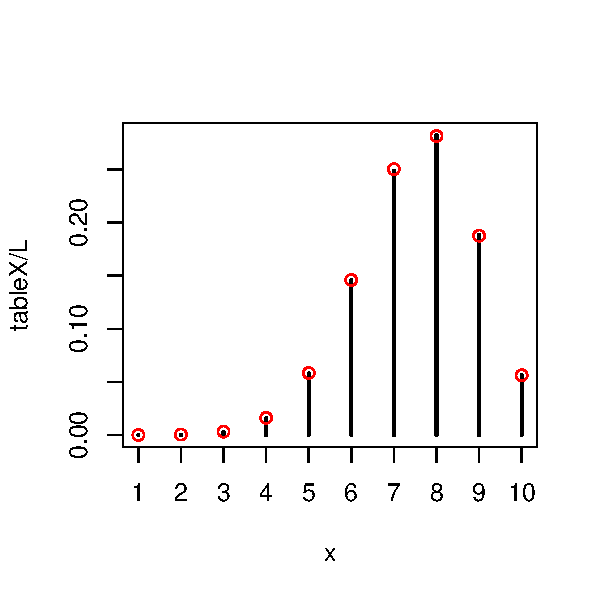
\includegraphics[width=.60\linewidth]{figure/histBinomial_} 

\end{knitrout}


Podemos calcular el valor esperado y varianza utilizando la función característica y sus derivadas. El resultado es
\begin{equation}\label{caracterBinomial}
  \begin{split}
    \phi_{X}(t) &= (p e^{it} + 1 - p )^{n} \\
    E[X] &= np\\
    \Var [X] &= np(1-p)\:.
  \end{split}
\end{equation}

\section{Distribucion Geométrica.}
Supongamos que un experimento se repite de manera independiente, con probabilidad de éxito $p$, hasta que se obtiene el primer éxito después de $X$ fracasos. Entonces
\begin{equation}\label{dbinomial}
  \begin{split}
    P(X=x) &= p (1-p)^x\:.
  \end{split}
\end{equation}
Esta es la \emph{distribución geométrica} con parametro $p$ y se denota $G(p)$. Las muestras se crean llamando \verb+ rgeom( L , p ) + .

\begin{knitrout}
\definecolor{shadecolor}{rgb}{0.969, 0.969, 0.969}\color{fgcolor}\begin{kframe}
\begin{alltt}
\hlcom{## parametros}
\hlstd{L} \hlkwb{<-} \hlnum{1e+05}
\hlstd{p} \hlkwb{<-} \hlnum{0.75}
\hlstd{x} \hlkwb{<-} \hlkwd{rgeom}\hlstd{(L, p)}
\end{alltt}
\end{kframe}
\end{knitrout}

\begin{knitrout}
\definecolor{shadecolor}{rgb}{0.969, 0.969, 0.969}\color{fgcolor}\begin{kframe}
\begin{alltt}
\hlstd{tableX} \hlkwb{<-} \hlkwd{table}\hlstd{(x)}
\hlstd{f} \hlkwb{<-} \hlkwa{function}\hlstd{(}\hlkwc{x}\hlstd{) p}\hlopt{*}\hlstd{(}\hlnum{1}\hlopt{-}\hlstd{p)}\hlopt{^}\hlstd{(x)}
\hlkwd{plot}\hlstd{(tableX}\hlopt{/}\hlstd{L)}
\hlstd{xNames} \hlkwb{<-} \hlkwd{as.numeric}\hlstd{(}\hlkwd{names}\hlstd{(tableX))}
\hlkwd{points}\hlstd{( xNames ,} \hlkwd{f}\hlstd{(xNames) ,} \hlkwc{col} \hlstd{=} \hlstr{"red"}\hlstd{)}
\end{alltt}
\end{kframe}
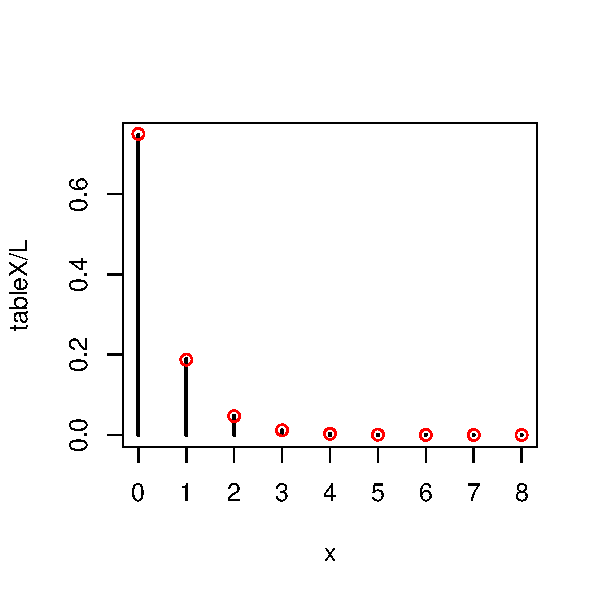
\includegraphics[width=.60\linewidth]{figure/histGeometrica_} 

\end{knitrout}

Podemos calcular el valor esperado y varianza utilizando la función característica y sus derivadas. El resultado es
\begin{equation}\label{caracterGeometrica}
  \begin{split}
    \phi_{X}(t) &= \frac{p}{1-(1-p)e^{it}} \\
    E[X] &= (1-p)/p\\
    \Var [X] &= (1-p)/p^2\:.
  \end{split}
\end{equation}

\section{Distribución de Poisson}
Supongamos que tenemos $n$ personas aseguradas y que cada una de ellas tiene la misma probabilidad $p$ de sufrir un accidente en el primer año de coberture de manera independiente. Denotemos por $X$ el número total de accidentes sufridos por las $n$ personas aseguradas en el primer año y supongamos que  $X$ tiene valor esperado $\lambda$.

La v.a. $X$ tiene distribución $N(n,p)$ y por lo tanto $\lambda = np$, es decir $p = \lambda/n$. La función de densidad de $X$ es
\begin{equation}
  \begin{split}
    f_{n}(x)&= { n \choose x } \biggl( \frac{\lambda}{n} \biggr)^{x} \biggl( 1-\frac{\lambda}{n} \biggr)^{n-x}\\
        &=\frac{n!}{x!(n-x)!}\frac{\lambda^{x}(n-\lambda)^{n-x}}{n^x n^{n-x}}\\
        &=\frac{n!}{(n-x)!(n-\lambda)^x}\frac{\lambda^{x}}{x!}\biggl( 1-\frac{\lambda}{n}\biggr)^{n}\\
        &=\frac{n(n-1)\cdots (n-x+1)}{(n-\lambda)^x}\frac{\lambda^{x}}{x!}\biggl( 1-\frac{\lambda}{n}\biggr)^{n}
  \end{split}
\end{equation}
Se deja como ejercico de cálculo el mostra que
\begin{equation}
  \begin{split}
    \lim_{n\to\infty}\frac{n(n-1)\cdots (n-x+1)}{(n-\lambda)^x}&=1\\
    \lim_{n\to\infty} \biggl( 1-\frac{\lambda}{n}\biggr)^{n} &= e^{-\lambda}\:.
  \end{split}
\end{equation}
La función de densidad límite
\begin{equation}\label{dpoisson}
  \begin{split}
    f(x) &= e^{-\lambda}\frac{\lambda^{x}}{x!}\:,
  \end{split}
\end{equation}
es la función de densidad de una v.a. con \emph{distribución de Poisson con parámetro $\lambda$}. Podemos calcular el valor esperado y la varianze como sigue.
\begin{equation}
  \begin{split}
    E[X] &= \lambda\\
    \Var [X] &= \lambda \\
  \end{split}
\end{equation}
Las muestras se crean llamando \verb+ rpois( L , lambda ) + .
\begin{knitrout}
\definecolor{shadecolor}{rgb}{0.969, 0.969, 0.969}\color{fgcolor}\begin{kframe}
\begin{alltt}
\hlcom{## parametros}
\hlstd{L} \hlkwb{<-} \hlnum{1e+05}
\hlstd{lambda} \hlkwb{<-} \hlnum{10}
\hlstd{x} \hlkwb{<-} \hlkwd{rpois}\hlstd{(L, lambda)}
\end{alltt}
\end{kframe}
\end{knitrout}

\begin{knitrout}
\definecolor{shadecolor}{rgb}{0.969, 0.969, 0.969}\color{fgcolor}\begin{kframe}
\begin{alltt}
\hlstd{tableX} \hlkwb{<-} \hlkwd{table}\hlstd{(x)}
\hlstd{f} \hlkwb{<-} \hlkwa{function}\hlstd{(}\hlkwc{x}\hlstd{)} \hlkwd{exp}\hlstd{(}\hlopt{-}\hlstd{lambda)}\hlopt{*}\hlstd{lambda}\hlopt{^}\hlstd{(x)}\hlopt{/}\hlkwd{factorial}\hlstd{(x)}
\hlkwd{plot}\hlstd{(tableX}\hlopt{/}\hlstd{L)}
\hlstd{xNames} \hlkwb{<-} \hlkwd{as.numeric}\hlstd{(}\hlkwd{names}\hlstd{(tableX))}
\hlkwd{points}\hlstd{( xNames ,} \hlkwd{f}\hlstd{(xNames) ,} \hlkwc{col} \hlstd{=} \hlstr{"red"}\hlstd{)}
\end{alltt}
\end{kframe}
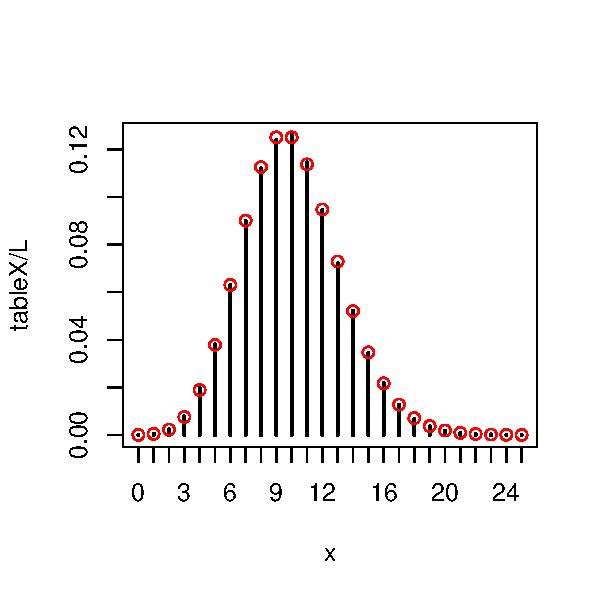
\includegraphics[width=.60\linewidth]{figure/histPoisson_} 

\end{knitrout}



\section{Distribución exponencial}
La distribución exponencial con parámetro $\lambda$ tiene función de densidad
\begin{equation}\label{dexp}
  \begin{split}
  f(t)&= \lambda \exp(-\lambda t),\qquad t > 0 \:,
  \end{split}
\end{equation}

y función de distribución
\begin{equation}\label{pexp}
  \begin{split}
  F(t)&= 1-\exp(-\lambda t),\qquad t > 0 \:.
  \end{split}
\end{equation}
Su valor esperado y varianza se pueden calcular utilizando la función característica. El resultado es
\begin{equation}\label{mexp}
  \begin{split}
  \phi_{X}(t) &= \biggl( 1 - i \frac{t}{\lambda} \biggr)^{-1} \\
  E[T] &= \frac{1}{\lambda}\\
  \Var [T] &=\frac{1}{\lambda^2} \\
  \end{split}
\end{equation}
Esta distribución se utiliza para modelar tiempos de espera. Una propiedad deseable para la distribución de un tiempo de espera es que el tiempo de espera sea el mismo sin importar el tiempo que se ha esperado. En notación de probabilidades condicionales esto se escribe
\begin{equation}\label{prop_exp}
  \begin{split}
    P(T \leq t | T > s ) &= P( T \leq t-s)\\
    \frac{P(T \leq t , T > s )}{P(T>s)} &= P( T \leq t-s)\\
    \frac{\int_{s}^{t} f(x) dx}{\int_{s}^{\infty}f(x)dx} &= \int_{0}^{t-s}f(x)dx\:.
  \end{split}
\end{equation}
Tomamos la derivada con respecto de $t$ en la ecuación anterior para obtener
\begin{equation}
  \begin{split}
    \frac{f(t)}{\int_{s}^{\infty}f(x)dx} &= f(t-s)\\
    f(t)&= f(t-s)\int_{s}^{\infty}f(x)dx\\
  \end{split}
\end{equation}
Finalmente tomamos la derivada con respecto de $s$ en la ecuación anterior para obtener
\begin{equation}
  \begin{split}
    0 &= -f'(t-s)\int_{s}^{\infty}f(x)dx -f(t-s)f(s) \:,
  \end{split}
\end{equation}
y evaluando en $s=0$ la ecuación anterior se convierte en
\begin{equation}
  \begin{split}
    f'(t) &=-f(0)f(t) ,\qquad t>0\:.
  \end{split}
\end{equation}
La solución de la ecuación diferencial anterior es $f(t)=C\exp(-f(0)t)$ y si denotamos $\lambda=f(0)$ obtenemos que $C=\lambda$.

\begin{knitrout}
\definecolor{shadecolor}{rgb}{0.969, 0.969, 0.969}\color{fgcolor}\begin{kframe}
\begin{alltt}
\hlcom{## parametros}
\hlstd{L} \hlkwb{<-} \hlnum{10000}
\hlstd{lambda} \hlkwb{<-} \hlnum{2}
\hlstd{x} \hlkwb{<-} \hlkwd{rexp}\hlstd{(L, lambda)}
\end{alltt}
\end{kframe}
\end{knitrout}

\begin{knitrout}
\definecolor{shadecolor}{rgb}{0.969, 0.969, 0.969}\color{fgcolor}\begin{kframe}
\begin{alltt}
\hlstd{xHist} \hlkwb{<-} \hlkwd{hist}\hlstd{(x,} \hlkwc{prob} \hlstd{=} \hlnum{TRUE} \hlstd{,} \hlkwc{breaks} \hlstd{=} \hlnum{10}\hlopt{*}\hlkwd{log}\hlstd{(L))}
\hlstd{f} \hlkwb{<-} \hlkwa{function}\hlstd{(}\hlkwc{x}\hlstd{) lambda}\hlopt{*}\hlkwd{exp}\hlstd{(}\hlopt{-}\hlstd{lambda} \hlopt{*}\hlstd{x )}
\hlkwd{curve}\hlstd{( f , xHist}\hlopt{$}\hlstd{mids[}\hlnum{1}\hlstd{] , xHist}\hlopt{$}\hlstd{mids[}\hlkwd{length}\hlstd{(xHist}\hlopt{$}\hlstd{mids)] ,}
       \hlkwc{add} \hlstd{=} \hlnum{TRUE}\hlstd{,} \hlkwc{col} \hlstd{=} \hlstr{'red'}\hlstd{)}
\end{alltt}
\end{kframe}
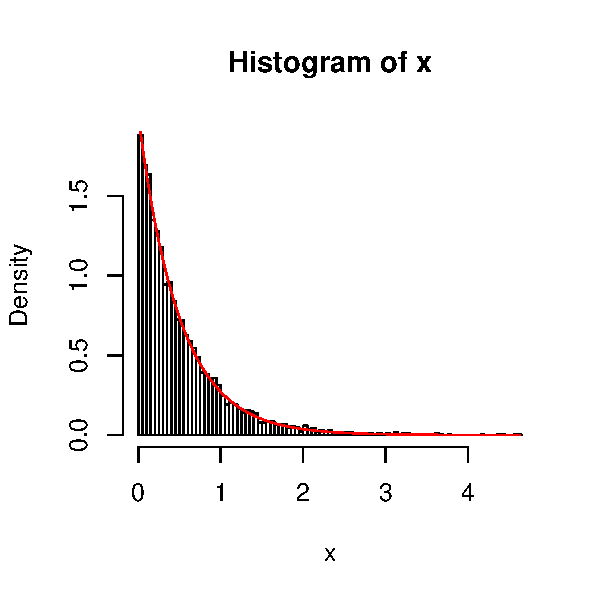
\includegraphics[width=.60\linewidth]{figure/histExp_} 

\end{knitrout}


\section{Distribución de Rayleigh}
La función de densidad es
\begin{equation}\label{dRayleigh}
  \begin{split}
    f(x) &= \frac{x}{\sigma^2} e^{-\frac{x^2}{2\sigma^2}}\:
  \end{split}
\end{equation}
Es complicado calcular la función característica, así que solo calculamos la media y la varianza. El resultado es
\begin{equation}\label{meanRayleigh}
  \begin{split}
    E[X] &= \sigma \sqrt{\frac{\pi}{2}} \\\
    E[X^2] &= 2 \sigma^2 \\
    \Var [X] &= \sigma^2 \biggl(2-\frac{\pi}{2}\biggr)
  \end{split}
\end{equation}

Desafortunadamente no hay generador de muestras para esta distribución en la instalación usual de \verb+R+. Sin embargo, podemos utilizar el \emph{método de la transformada inversa} para generar las muestras. La idea es simple: si $U_1$ es una muestra de la distribución uniforme en el intervalo $(0,1)$, entonces $X_1 = F_{X}^{-1}(U_1)$ es una muestra de $X$. Dejando la justificación del método como ejercicio, nos enfocamos en los cálculos necesarios.

Usando un cambio de variable podemos integrar la función de densidad en \eqref{dRayleigh} y obtener
\begin{equation}\label{cRayleigh}
  \begin{split}
  F_{X}(x) &= \begin{cases}
  1 - e^{-\frac{x^2}{2\sigma^2}} ,& \qquad x \geq 0 \\
  0 ,& \qquad x < 0 \\
  \end{cases}\\
  F_{X}^{-1}(u) &= \sqrt{-2 \sigma^2 \ln(1-u)}\:.
  \end{split}
\end{equation}

\begin{knitrout}
\definecolor{shadecolor}{rgb}{0.969, 0.969, 0.969}\color{fgcolor}\begin{kframe}
\begin{alltt}
\hlcom{## parametros}
\hlstd{L} \hlkwb{<-} \hlnum{1e+05}
\hlstd{sigma} \hlkwb{<-} \hlnum{1}
\hlstd{u} \hlkwb{<-} \hlkwd{runif}\hlstd{(L)}
\hlstd{x} \hlkwb{<-} \hlkwd{sqrt}\hlstd{(}\hlopt{-}\hlnum{2} \hlopt{*} \hlstd{sigma} \hlopt{*} \hlstd{sigma} \hlopt{*} \hlkwd{log}\hlstd{(}\hlnum{1} \hlopt{-} \hlstd{u))}
\end{alltt}
\end{kframe}
\end{knitrout}

\begin{knitrout}
\definecolor{shadecolor}{rgb}{0.969, 0.969, 0.969}\color{fgcolor}\begin{kframe}
\begin{alltt}
\hlstd{xHist} \hlkwb{<-} \hlkwd{hist}\hlstd{(x,} \hlkwc{prob} \hlstd{=} \hlnum{TRUE} \hlstd{,} \hlkwc{breaks} \hlstd{=} \hlnum{10}\hlopt{*}\hlkwd{log}\hlstd{(L))}
\hlstd{f} \hlkwb{<-} \hlkwa{function}\hlstd{(}\hlkwc{x}\hlstd{) (x}\hlopt{/}\hlstd{(sigma}\hlopt{*}\hlstd{sigma))}\hlopt{*}\hlkwd{exp}\hlstd{(}\hlopt{-}\hlstd{x}\hlopt{*}\hlstd{x}\hlopt{/}\hlstd{(}\hlnum{2.0}\hlopt{*}\hlstd{sigma}\hlopt{*}\hlstd{sigma) )}
\hlkwd{curve}\hlstd{( f , xHist}\hlopt{$}\hlstd{mids[}\hlnum{1}\hlstd{] , xHist}\hlopt{$}\hlstd{mids[}\hlkwd{length}\hlstd{(xHist}\hlopt{$}\hlstd{mids)] ,}
       \hlkwc{add} \hlstd{=} \hlnum{TRUE}\hlstd{,} \hlkwc{col} \hlstd{=} \hlstr{'red'}\hlstd{)}
\end{alltt}
\end{kframe}
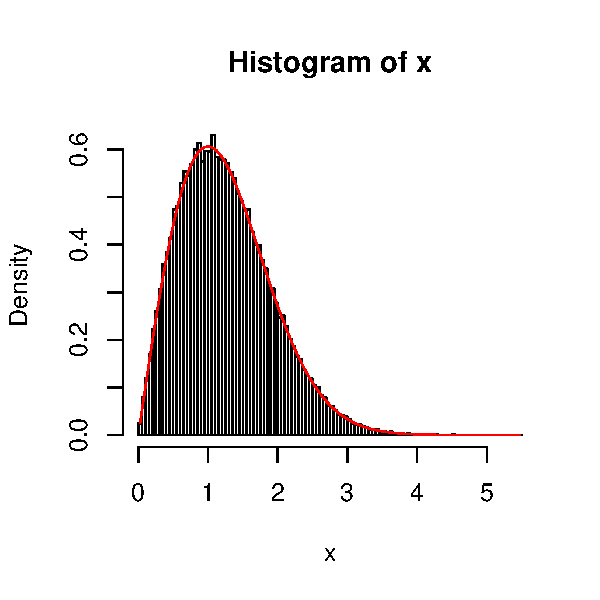
\includegraphics[width=.60\linewidth]{figure/histRayleigh_} 

\end{knitrout}


\section{Distribución normal}
La distribución normal es la más importante en el el estudio de procesos estocásticos. Su ubicuidad se debe al teorema del límite central. Discutiremos esta relación más adelante en el curso y por lo pronto estudiaremos sus propiedades.

La variable aleatoria $X$ tiene distribución normal con media $\mu$ y varianza $\sigma^2$ si su función de densidad es 
\begin{equation}\label{denNormal}
  \begin{split}
  f(x) &= \frac{\exp(-\frac{(x-\mu)^2}{2 \sigma^2})}{\sqrt{2 \pi \sigma^2}}\:.
  \end{split}
\end{equation}
Escribiremos $X \sim N(\mu,\sigma^2)$ para denotar que la variable aleatoria $X$ tiene la densidad anterior. La función característica es
\begin{equation}\label{caracterNormal}
  \begin{split}
  \phi(t) &= \exp(i\mu t)\:\exp\biggl(-\frac{\sigma^2 t^2}{2}\biggr) \:.
  \end{split}
\end{equation}
El siguiente código genera 10,000 muestras $N(3,4)$ y dibuja el histograma. Nótese que en el lenguaje \verb+ R + el parámetro que se usa es la desviación estándar $\sigma$.
\begin{knitrout}
\definecolor{shadecolor}{rgb}{0.969, 0.969, 0.969}\color{fgcolor}\begin{kframe}
\begin{alltt}
\hlcom{## parametros}
\hlstd{L} \hlkwb{<-} \hlnum{10000}
\hlstd{mu} \hlkwb{<-} \hlnum{3}
\hlstd{sigma} \hlkwb{<-} \hlnum{2}
\hlstd{x} \hlkwb{<-} \hlkwd{rnorm}\hlstd{(L, mu, sigma)}
\end{alltt}
\end{kframe}
\end{knitrout}

\begin{knitrout}
\definecolor{shadecolor}{rgb}{0.969, 0.969, 0.969}\color{fgcolor}\begin{kframe}
\begin{alltt}
\hlstd{xHist} \hlkwb{<-} \hlkwd{hist}\hlstd{(x,} \hlkwc{prob} \hlstd{=} \hlnum{TRUE} \hlstd{,} \hlkwc{breaks} \hlstd{=} \hlnum{10}\hlopt{*}\hlkwd{log}\hlstd{(L))}
\hlstd{f} \hlkwb{<-} \hlkwa{function}\hlstd{(}\hlkwc{x}\hlstd{)} \hlkwd{exp}\hlstd{(}\hlopt{-} \hlstd{((x}\hlopt{-}\hlstd{mu)}\hlopt{^}\hlnum{2}\hlstd{)}\hlopt{/}\hlstd{(}\hlnum{2}\hlopt{*}\hlstd{sigma}\hlopt{^}\hlnum{2}\hlstd{))}\hlopt{/}\hlkwd{sqrt}\hlstd{(}\hlnum{2}\hlopt{*}\hlstd{pi}\hlopt{*}\hlstd{sigma}\hlopt{^}\hlnum{2}\hlstd{)}
\hlkwd{curve}\hlstd{( f , xHist}\hlopt{$}\hlstd{mids[}\hlnum{1}\hlstd{] , xHist}\hlopt{$}\hlstd{mids[}\hlkwd{length}\hlstd{(xHist}\hlopt{$}\hlstd{mids)] ,}
       \hlkwc{add} \hlstd{=} \hlnum{TRUE}\hlstd{,} \hlkwc{col} \hlstd{=} \hlstr{'red'}\hlstd{)}
\end{alltt}
\end{kframe}
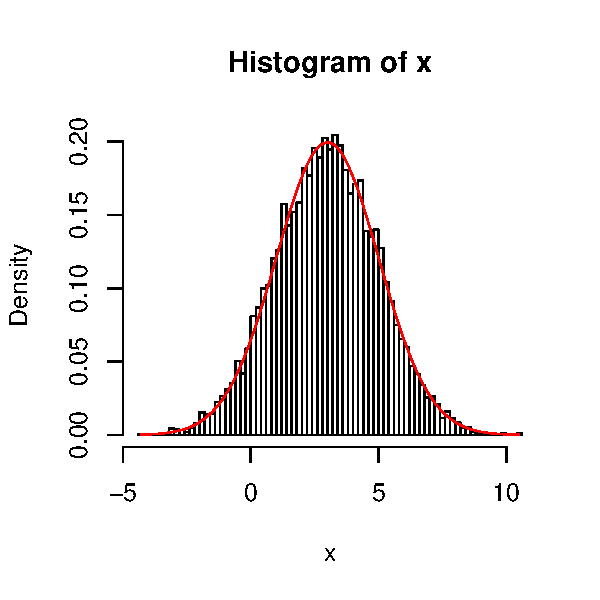
\includegraphics[width=.60\linewidth]{figure/histN_} 

\end{knitrout}


\section{Vectores aleatorios Gaussianos}

La distribución normal tiene una extensión natural para el caso de variables aleatorias correlacionadas. Supongamos que $Z_1,Z_2$ son variables aleatorias normales estándar independientes. Acomodamos las v.a. en un vector columna $Z = (Z_1,Z_2)^T$ y definimos un vector aleatorio $X$ mediante una transformación lineal $\sigma: \R^2 \to \R^2$, es decir $X = \sigma Z$. En términos de las coordenadas del vector $X$ tenemos
\begin{equation}\label{coordenadasX}
  \begin{split}
  X_1 &= \sigma_{11}Z_1 + \sigma_{12}Z_2\\
  X_2 &= \sigma_{21}Z_1 + \sigma_{22}Z_2\\
  \end{split}
\end{equation}
Las entradas de $X$ no son independientes porque en las sumas que las definen hay elementos repetidos. Podemos calcular la covarianza entre las entradas como sigue.
\begin{equation*}
  \begin{split}
  \Cov(X_1 ,X_2) &=\Cov(\sigma_{11}Z_1 + \sigma_{12}Z_2,\sigma_{21}Z_1 + \sigma_{22}Z_2 )\\
 &= \sum_{k,l}\sigma_{1k}\sigma_{2l}\Cov(Z_k,Z_l)
  \end{split}
\end{equation*}
Usando que las v.a. $Z_i$ son independientes y tienen varianza 1 obtenemos que
\begin{equation}\label{covarianzaX12}
  \begin{split}
  \Cov(X_1 ,X_2) &=\sum_{k}\sigma_{1k}\sigma_{2k}
  \end{split}
\end{equation}
La suma que aparece al final de la última ecuación es igual a la entrada $(1,2)$ de la matriz $\sigma\sigma^T$. Cálculos similares llevan a la conclusión de que la \emph{matriz de covarianza} de $X$ es $\Sigma = \sigma\sigma^T$. En otras palabras
\begin{equation}\label{covarianzaX}
  \begin{split}
  \Cov(X_i ,X_j) &=\sum_{k}\sigma_{ik}\sigma_{jk}=(\sigma\sigma^T)_{ij}\:.
  \end{split}
\end{equation}

También podemos calcular la función de densidad del vector $X$ de la siguiente forma.
\begin{enumerate}
\item Escribir la función de densidad de $Z$ en \emph{notación diferencial}.
\begin{equation}\label{density_z}
  \begin{split}
  f_{Z}(z) |dz| &= \frac{e^{-z_1^2/2}}{\sqrt{2\pi}}\frac{e^{-z_2^2/2}}{\sqrt{2\pi}} |dz_1 dz_2|\\
  &= \frac{e^{-\frac{1}{2}z^T z}}{\sqrt{2\pi}} |dz_1 dz_2|\:.
  \end{split}
\end{equation}
\item Sustituir $z_i$ y $dz_i$ en la ecuación anterior usando la relación $x = \sigma z$. 
Despejando $z$ obtenemos
\begin{equation}\label{z}
  \begin{split}
  z &= \sigma^{-1} x,  
  \end{split}
\end{equation}
Calculando el diferencial obtenemos
\begin{equation*}
  \begin{split}
  dx_1 &= \sigma_{11}dz_1 + \sigma_{12}dz_2\\
  dx_2 &= \sigma_{21}dz_1 + \sigma_{22}dz_2\:.
  \end{split}
\end{equation*}
Usando que $dz_1 dz_1=0$, $dz_2 dz_2=0$ y  $dz_1 dz_2 = - dz_2 dz_1$ calculamos
\begin{equation}\label{dz}
  \begin{split}
  dx_1 dx_2 &= \sigma_{11}\sigma_{22}dz_1 dz_2 + \sigma_{12}\sigma_{21} dz_2 dz_1\\
  &= (\sigma_{11}\sigma_{22}-  \sigma_{12}\sigma_{21})dz_1dz_2\\
  &= \det(\sigma) dz_1 dz_2\\
  \end{split}
\end{equation}
Finalmente sustituimos \eqref{z} y \eqref{dz} en la ecuación \eqref{density_z} para obtener
\begin{equation}\label{substitute_x}
  \begin{split}
  f_{Z}(z) |dz| &= \frac{e^{-\frac{1}{2}x^T(\sigma\sigma^T)^{-1}x}}{(\sqrt{2\pi})^2}\frac{1}{|\det{\sigma}|} |dx_1 dx_2|\:.
  \end{split}
\end{equation}
\item El factor enfrente de $|dx_1 dx_2|$ es la función de densidad de la variable aleatoria $X$, en otras palabras
\begin{equation}\label{density_x}
  \begin{split}
  f_{X}(x) &= \frac{e^{-\frac{1}{2}x^T(\sigma\sigma^T)^{-1}x}}{(\sqrt{2\pi})^2}\frac{1}{|\det{\sigma}|}\:.
  \end{split}
\end{equation}
\end{enumerate}
Usando propiedades básicas del determinante de una matriz podemos calcular
\begin{equation*}
  \begin{split}
  \det(\sigma \sigma^T) &= \det(\sigma) \det(\sigma^T)\\
  &= \det(\sigma) \det(\sigma)\\
  &= \det(\sigma)^2\:.
  \end{split}
\end{equation*}
En términos de la matriz $\Sigma$ hemos obtenido que
\begin{equation*}
  \begin{split}
  f_{X}(x) &= \frac{e^{-\frac{1}{2}x^T \Sigma ^{-1}x}}{(\sqrt{2\pi})^2}\frac{1}{\sqrt{\det{\Sigma}}}\:.
  \end{split}
\end{equation*}
En el caso multivariado donde $X\in \R^n$ y $\sigma:\R^n\To \R^n$ la ecuación anterior se convierte en
\begin{equation}\label{density_N}
  \begin{split}
  f_{X}(x) &= \frac{e^{-\frac{1}{2}x^T \Sigma ^{-1}x}}{(\sqrt{2\pi})^n\sqrt{\det{\Sigma}}}\:.
  \end{split}
\end{equation}
En este caso decimos que las entradas $X_i$ tienen una \emph{distribución normal conjunta} con media cero y covarianza $\Sigma$. Si queremos que $E[X_i]=\mu_i$ la función de densidad debe ser
\begin{equation}\label{density_N_mu}
  \begin{split}
  f_{X}(x) &= \frac{e^{-\frac{1}{2}(x-\mu)^T \Sigma ^{-1}(x-\mu)}}{(\sqrt{2\pi})^n\sqrt{\det{\Sigma}}}\:.
  \end{split}
\end{equation}

\end{document}
